\documentclass[a4paper,12pt]{article}

\usepackage[utf8]{inputenc}   % Codificação UTF-8
\usepackage[T1]{fontenc}      % Codificação da fonte
\usepackage{enumitem}
\usepackage{graphicx}
\usepackage{caption}
\usepackage{float}
\usepackage{pgffor}

\newcommand\Insert[1]{%
    \foreach \x in {#1}{%
        \begin{figure}[H]
            \centering
            \includegraphics[width=0.6\textwidth]{Aula03/Daniel/\x.png} % adjust path
            \caption*{\x} % <- custom caption (no "Figure" label, no numbering)
            \label{fig:Graphic\x} % still works for \ref if you want
        \end{figure}
    }%
}


\title{LFTC}
\author{Miguel de Campos R. Moret \\ Abigail Sayury Nakashima}
\date{\today}

\begin{document}

\maketitle
\newpage

\tableofcontents
\newpage

\section{Aula 02 }
    \subsection{Descreva as linguagens denotadas pelas ER’s abaixo sobre o alfabeto $\sum = \{0,1\}$.}
    \begin{enumerate}[label=\textbf{\alph* -}]
        \item $\mathbf{0|10^*}$
            \\ A linguagem é composta por cadeias que contêm apenas o símbolo $0$ ou que iniciam com $1$ seguido de qualquer quantidade (inclusive zero) de $0$'s.
        \item $\mathbf{(0|1)0^*}$
            \\ A linguagem é composta por cadeias que iniciam com $0$ ou com $1$ e são seguidos por qualquer quantidade (inclusive zero) de $0$'s.
        \item $\mathbf{(0011)^*}$
            \\ A linguagem é composta por cadeias compostas por qualquer quan\-tidade (inclusive zero) da substring "$0011$".
        \item $\mathbf{(0|1)^*1(0|1)^*}$
            \\ A linguagem é composta por cadeias que contem pelo menos um $1$.
        \item $\mathbf{0^*11^*0}$
            \\ A linguagem é composta por cadeias que iniciam com qualquer quan\-tidade (inclusive zero) de $0$'s, segiodos por pelo menos um $1$, finalizando com um único símbolo $0$.
        \item $\mathbf{0(0|1)^*0}$
            \\ A linguagem é composta por cadeias que iniciam e  terminam com $0$.
        \item $\mathbf{(\epsilon+0)(\epsilon|1)}$
            \\ A linguagem é composta por 4 cadeias diferentes: uma cadeia sem símbolos ("vazia"), uma cadeia composta por um único $0$, uma cadeia composta por um único $1$ e uma cadeia composta por um $0$ seguido por um $1$.
        \item $\mathbf{(000^*|1)^*}$
            \\ A linguagem é composta por cadeias que não contêm $0$'s sozinhos (eles estão sempre em grupos de $2+$).
        \item $\mathbf{(0^*|0^*11(1|00^*11)^*)(\epsilon|00^*)}$
            \\ A linguagem de todas as cadeias em que cada bloco de 1’s tem comprimento pelo menos 2.
    \end{enumerate}

    \subsection{Sobre o $\sum = \{a,b\}$, defina expressoes regulares que representam as linguagens cujas sentencas estao descritas a seguir} 
    \begin{itemize}
        \item \textbf{Possuem comprimento maior ou igual a 3;}
            \\ $(a|b)(a|b)(a|b)(a|b)*$
        \item \textbf{Possuem comprimento menor ou igual a 3;}
            \\ $*(a|b|\epsilon)(a|b|\epsilon)(a|b|\epsilon)$
        \item \textbf{Possuem comprimento diferente a 3;}
            \\ $((a|b|\epsilon)(a|b|\epsilon))|((a|b)(a|b)(a|b)(a|b)*)$
        \item \textbf{Possuem comprimento par;}
            \\ $((a|b)(a|b))^*$
        \item \textbf{Possuem comprimento impar;}
            \\ $(a|b)((a|b)(a|b))^*$
        \item \textbf{Possuem comprimento multiplo de 4;}
            \\ $(a|b)(a|b)(a|b)(a|b)((a|b)(a|b)(a|b)(a|b))^*$
    \end{itemize}

    \subsection{Fazer o conjunto de exercícios da seção 3.1 do livro do HOPCROFT, páginas 96 e 97.} 
        \subsubsection{Escreva expressões regulares corresponden\-tes às seguintes linguagens:}
            \begin{enumerate}[label={\bfseries \alph*)}]
                \item O conjunto de strings sobre o alfabeto $\{a, b, c\}$ que contém pelo menos um $a$ e um $b$.
                    \\ $((c|a|b)^* a(c|a|b)^* b(c|a|b)^*)|((c|a|b)^* b(c|a|b)^* a(c|a|b)^*)$.
                \item O conjunto de strings $0$'s e $1$'s cujo décimo símbolo a partir da extremidade direita é $1$.
                    \\ $(0|1)^* 1 (0|1)(0|1)(0|1)(0|1)(0|1)(0|1)(0|1)(0|1)(0|1)$.
                \item O conjunto de strings $0$'s e $1$'s com no máximo um par de $1$'s consecutivos.
                    \\ $(0|10)^*(11)?(0|01)^*$
            \end{enumerate}
            
        \subsubsection{Escreva expressões regulares corresponden\-tes às seguintes linguagens:}
            \begin{enumerate}[label={\bfseries \alph*)}]
                \item O conjunto de todos os strings de $0$'s e $1$'s tais que todo par de $0$'s adjacentes aparece antes de qualquer par de $1$'s adjacentes.
                    \\ $(1^*(01)^*)^*(00)^*(0^*(10)^*)^*(11)^*(1^*(01)^*)^*$
                \item O conjunto de strings $0$'s e $1$'s cujo número de $0$'s é divisível por $5$.
                    \\ $(1^*01^*01^*01^*01^*0)(1^*01^*01^*01^*01^*0)^*$
            \end{enumerate}
        
        \subsubsection{Escreva expressões regulares corresponden\-tes às seguintes linguagens:}
            \begin{enumerate}[start=1, label={\bfseries \alph*)}]
                \item O conjunto de todos os strings $0$'s e $1$'s que não contêm $101$ como um substring.
                    \\ $(0^*|1^*)(0^*|1^*)(0^*00(1^*)|0^*)^*$
                \item O conjunto de todos os strings com um número igual de $0$'s e $1$'s, tais que nenhum prefixo tenha dois $0$'s a mais que os $1$'s, nem dois $1$'s a mais que os $0$'s.
                    \\ $(01|10|0011|1100|1001|0110)*$
                \item O conjunto de strings de $0$'s e $1$'scujo número de $0$'s é divisível por $5$ e cujo número de $1$'s é par.
                    \\ $((11)^*0(11)^*0(11)^*0(11)^*0(11)^*0)((11)^*0(11)^*0(11)^*0(11)^*0(11)^*0)^*$
            \end{enumerate}
        
            \subsubsection{Forneça descrições em português das linguagens correspon\-dedentes às seguintes expressões regulares:}
            \begin{enumerate}[label={\bfseries \alph*)}]
                \item $\mathbf{(1+\epsilon)(00^*)^*0^*}$.
                    \\ Linguagem de todas as cadeias com $\sum=\{0,1\}$ que são ou vazias, ou contém somente zeros, ou possuem um único $1$ seguido por múltiplos (ou nenhum) $0$'s.
                \item $\mathbf{(0^*1^*)^*000(0+1)^*}$.
                    \\ Linguagem de todas as cadeias com $\sum=\{0,1\}$ que contêm “000” como substring.
                \item $\mathbf{(0+10)^*1^*}$.
                    \\ Linguagem de todas as cadeias com $\sum=\{0,1\}$ que contêm pares $11$ somente no final da cadeia.
            \end{enumerate}

            \subsubsection{No Exemplo 3.1, destacamos que $\emptyset$ é uma das duas linguagens cujo fechammento é finito. Qual é a outra?}
                A outra linguagem é $\mathbf{\epsilon}$

\section{Aula 03 - Feito junto de Daniel Padua}

    \foreach \i in {1,...,11}{
    \begin{figure}[H] 
        \centering
        \includegraphics[width=0.5\textwidth]{Aula03/Daniel/\i.png}
        \caption*{\i}
    \end{figure}
    }
    \foreach \i in {15,...,19}{
    \begin{figure}[H] 
        \centering
        \includegraphics[width=0.5\textwidth]{Aula03/Daniel/\i.png}
        \caption*{\i}
    \end{figure}
    }
    \foreach \i in {20,...,29}{
    \begin{figure}[H]
        \centering
        \includegraphics[width=0.5\textwidth]{Aula03/Abigail/\i.png}
        \caption*{\i}
    \end{figure}
    }


$30) G = ({S,A}, {a,b,c}, P, S)$ \\
$P = { S-> aS | bA | cS | e,
A -> aA | bS | cA
}$ \\

$31) G = ({S,A}, {a,b,c}, P, S)$ \\
    $P = { S-> aS | bS | cA | c,
    A -> aA | bA | cS | e
    }$ \\

$32) G = ({S,A,B,C}, {a,b,c}, P, S)$ \\
    $P = { 
    S -> aB | bS | cA,
    A -> aC | bA | cS | e,
    B -> aS | bB | cC,
    C -> aA | bC | cB
    }$ \\
    
$33) G = ({S,A}, {a,b,c}, P, S)$ \\
    $P = { 
        S -> aS | bS | cS | abcA \\
        A -> e,
        }$ \\
        
        $34) G = ({S,A,B,C,D}, {a,b,c}, P, S)$ \\
        $P = { 
            S -> aS | bS | cS | aA | bB | cC, \\
            A -> aaS | aaD, \\
            B -> bbS | bbD, \\
            C -> ccS | ccD, \\
            D -> aD | bD | cD | e, \\
            }$ \\
            
            $35) G = ({S,A,B,C}, {a,b,c}, P, S)$ \\
            $P = { 
                S -> A | B | C | e, \\
                A -> bB | CC | e, \\
                B -> aA | cC | e, \\
                C -> bB | cC | e \\
                }$ \\
                
                $36) G = ({S}, {a,b,c}, P, S)$ \\
                $P = { 
                    S -> bS | cS | e,
                    }$ \\
                    
                    $37) G = ({S, A}, {a,b,c}, P, S)$ \\
                    $P = { 
                        S -> aA |bS | cS | e, \\
                        A -> aA | cS | e \\
                        }$ \\
                        
                        $38) G = ({S, A}, {a,b,c}, P, S)$ \\
                        $P = { 
                            S -> aA | bS | cS | e, \\
                            A -> aA | bB | cS | e, \\
                            B -> aA | bS | e \\
                            }$ \\
                            
                            \newpage
                            expressoes regulares:
                            \begin{figure}[H]
                                \centering
                                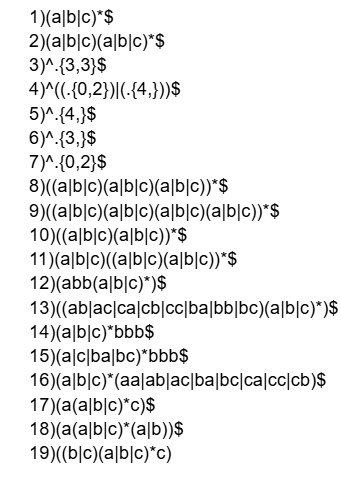
\includegraphics[width=0.6\textwidth]{Aula03/Daniel/ER.png}
                                \caption*{1-19}
                            \end{figure}
                            
    $30) ((a|c)*((a|c)*b(a|c)*b)*)*$ \\
                            
    $31) [ab]*c([ab]*c[ab]*c)*[ab]*$ \\
                            
    $32) (b*(ab*ab*)*cb*(ab*ab*)*)|(b*(ab*ab*)*ab*cb*(ab*ab*)*ab*)(c[(b*(ab*ab*)*cb*(ab*ab*)*)|(b*(ab*ab*)*ab*cb*(ab*ab*)*ab*)])*$ \\
                            
    $33) [ac]*abc[ac]*$ \\
                            
    $34) [ac]*(aaa|bbb|ccc)[ac]*$ \\
    
    $35) (a(b|c)|b(a|c)|c(a|b))*$ \\
    
    $36) (b|c|a(a|c)?)*$ \\
    
    $37) (b|c|a(b|a|c)?)*$ \\
    
    $38) (b|c|a(b|a|c)?)*$ \\
    
\section{Aula 04}
    \foreach \i in {1,...,18}{
    \begin{figure}[H]
        \centering
        \includegraphics[width=0.5\textwidth]{Aula04/\i.png}
        \caption*{\i}
    \end{figure}
    }

\end{document}